\section{Results}
\label{sec:results}

\begin{figure*}
    \begin{minipage}{0.33\textwidth}
        \centering
        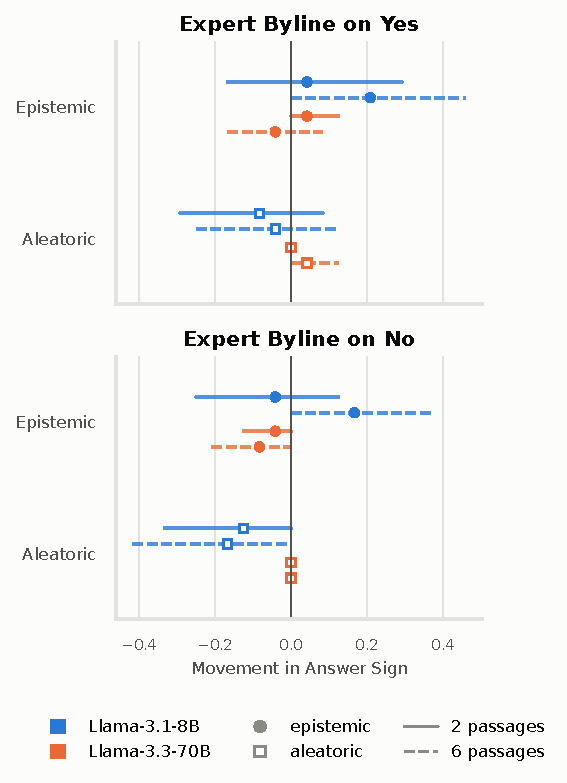
\includegraphics[width=\linewidth]{images/byline_balanced.pdf}
        \subcaption{Results for byline perturbation.}
        \label{fig:byline_balanced}
    \end{minipage}
    \begin{minipage}{0.33\textwidth}
        \centering
        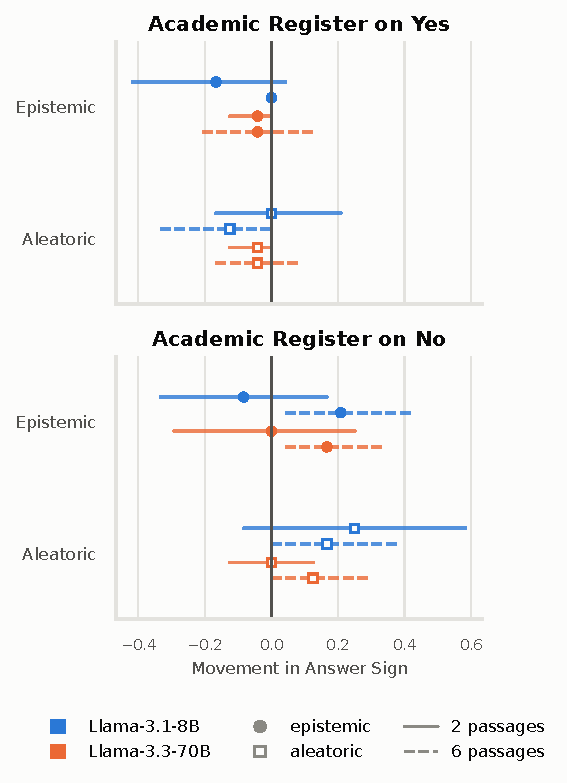
\includegraphics[width=\linewidth]{images/register_balanced.pdf}
        \subcaption{Results for register perturbation.}
        \label{fig:register_balanced}
    \end{minipage}
    \begin{minipage}{0.33\textwidth}
        \centering
        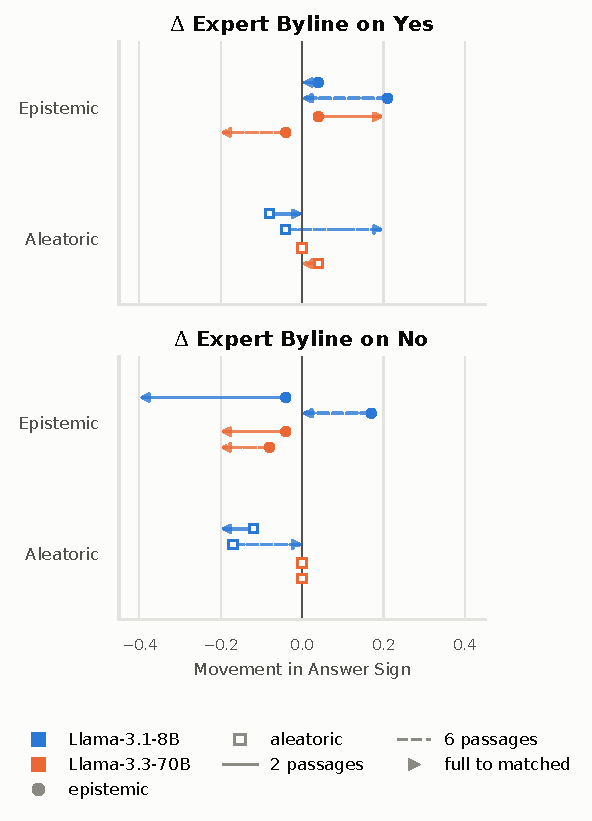
\includegraphics[width=\linewidth]{images/matched.pdf}
        \subcaption{$\Delta$ byline effect for shared categories.}
        \label{fig:matched}
    \end{minipage}
    \caption{Expertise and rhetorical authority perturbation. The first two panels show the byline and register perturbations. Solid lines give results with one passage per side; dashed lines give results with three passages per side. The same questions are used at both evidence sizes. The third panel restricts the questions to categories that contain both epistemic and aleatoric questions and applies the byline perturbation; only ten questions pass this filter. Filled icons mark the matched condition, hollow icons the full set of selected questions. In all three panels, the x-axis shows movement towards \emph{yes} (positive) or towards \emph{no} (negative).}
    \label{fig:expertise_results}
\end{figure*}

Figure~\ref{fig:expertise_results} shows results for the first experiment, which manipulates expertise signals. Models privilege expertise inconsistently, and the pattern depends on model size. The smaller model favours expert bylines on both epistemic and aleatoric questions, more strongly on the epistemic ones, and the effect grows as more passages support each answer. The larger model shows no significant movement under the byline perturbation.

The academic register reverses direction unexpectedly. Applied to the \emph{yes} passages, it moves neither model significantly towards \emph{yes}; applied to the \emph{no} passages, it moves both models significantly towards \emph{yes}. The expert byline produces the same reversal in the smaller model, which moves significantly towards \emph{yes} when the byline is applied to the \emph{no} passages.

As we discuss in Appendix~\ref{appendix_sub:prompts}, the \emph{yes} passages always appear first, followed by the \emph{no} passages. The lost-in-the-middle effect, compounded by the recency effect, may explain this asymmetry \citep{liu-etal-2024-lost,veseli2025positional,yi-etal-2026-attention}. In the 8B model, many prompts approach the maximum context window (see Appendices~\ref{appendix_sub:models} and~\ref{appendix_sub:prompts} for context windows and prompt sizes), which would account for effect sizes exceeding those of the 70B model. However, this does not explain why the register perturbation on the \emph{no} passages moves answers towards \emph{yes}. A second confound is the uneven distribution of questions across categories (see Appendix~\ref{appendix_sub:dataset}), since the register perturbation may act differently from one category to the next.

Figure~\ref{fig:matched} restricts the questions to categories that contain both epistemic and aleatoric questions. Only ten questions pass this filter, so we draw no strong conclusions, but the inconsistencies between the two question types persist. Both Figures~\ref{fig:byline_balanced} and~\ref{fig:matched}, for instance, show that the expert byline on the \emph{yes} passages moves answers towards \emph{no} in both models. Separating the features that contribute to these inconsistencies requires an evaluation set balanced across categories, with enough questions of each type in each, and across multiple presentation conditions (see Section~\ref{sec:discussion}).

\begin{figure}[ht!]
    \centering
    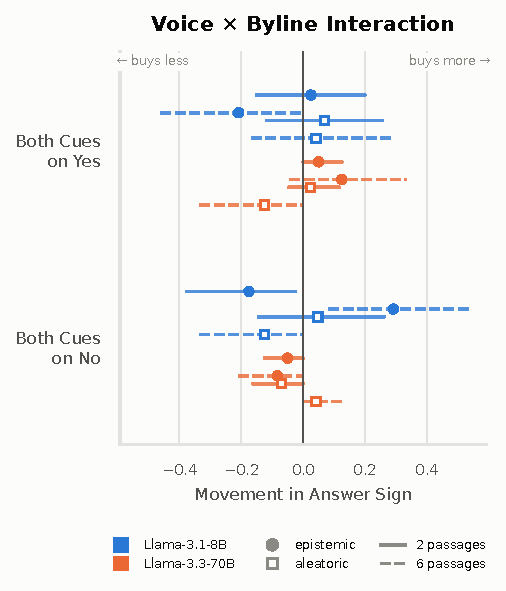
\includegraphics[width=0.75\linewidth]{images/register_byline_interaction.pdf}
    \caption{Interaction between register and byline perturbations.}
    \label{fig:register_byline_interaction}
\end{figure}

The two perturbations also interact. Figure~\ref{fig:register_byline_interaction} shows that they compound inconsistently across models and evidence directions. The smaller model compounds them for epistemic questions when more passages support the \emph{no} perspective; the larger model does so for the \emph{yes} perspective. For aleatoric questions the interaction appears to reverse, pushing the model away from the expert perspective. That reversal may reflect appropriate discounting of expertise on aleatoric questions, or one more artefact of presentation; distinguishing the two requires further investigation.

\section{Discussion}
\label{sec:discussion}

\begin{figure}
    \centering
    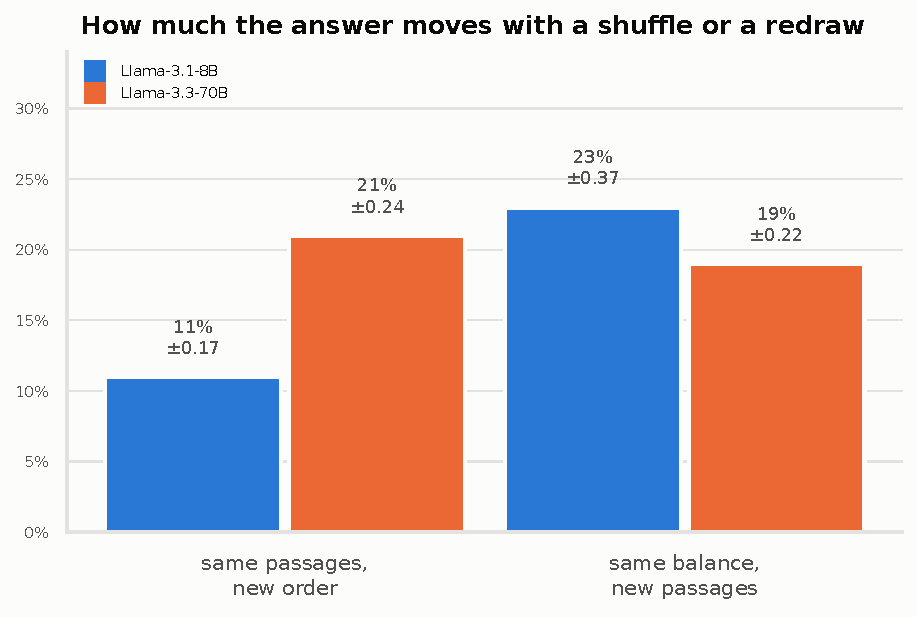
\includegraphics[width=0.85\linewidth]{images/stability.pdf}
    \caption{Instability under passage order and selection perturbations.}
    \label{fig:stability}
\end{figure}

Where evidence sits in the prompt strongly affects the model's answer. This is a known limitation of RAG systems \citep{liu-etal-2024-lost,veseli2025positional,yi-etal-2026-attention,naphade-2026-rational}, and it bears directly on the pluralistic groundedness of their answers. We ran two further experiments: one shuffled the order of the passages under five random seeds, the other re-drew the sample of passages for each answer. Figure~\ref{fig:stability} shows that the answers are unstable under both perturbations. The smaller model is more sensitive to passage selection, the larger model to passage order. The instability originates in the retrieval layer, but the aggregation layer may yet absorb it: a system could ensemble over passage orders at inference, or route evidence through separate perspective-specific models and combine their outputs \citep{feng-etal-2024-modular}. The pre-generation aggregation step is therefore worth addressing directly. Given a set of retrieved documents, can we rank them so as to produce fairer, more question-aware generation?

This instability clouds the results above, since separating the effects of passage order and selection from those of expertise signals will take further experiments. Even so, the inconsistency of the byline and register perturbations across models and question types suggests that models are \emph{sensitive} to expertise signals without being aligned with human judgements of expertise, and their compounding under larger evidence sets indicates that models grow more sensitive to register as evidence accumulates. Two design directions follow. A system could classify question type before aggregating, routing epistemic and aleatoric questions to different weightings instead of applying one rule to both. Evaluation could then audit that aggregation against social choice properties rather than win rate alone, which rewards agreement with a single passage and says nothing about how several passages combine.

Further work must also establish how multiple social choice features should interact. We limit our experiment to one feature, but on aleatoric questions a single principle will rarely prove authoritative. On a question about Buddhism, should a practising Buddhist's opinion outweigh that of a Christian who studies Buddhism? On whether to give children sweets on particular days, should a parent's opinion outweigh a non-parent's?